\chapter[Casos de Uso]{Casos de Uso}

\section{Diagrama de Casos de Uso}

\begin{figure}[H]
	\begin{center}
		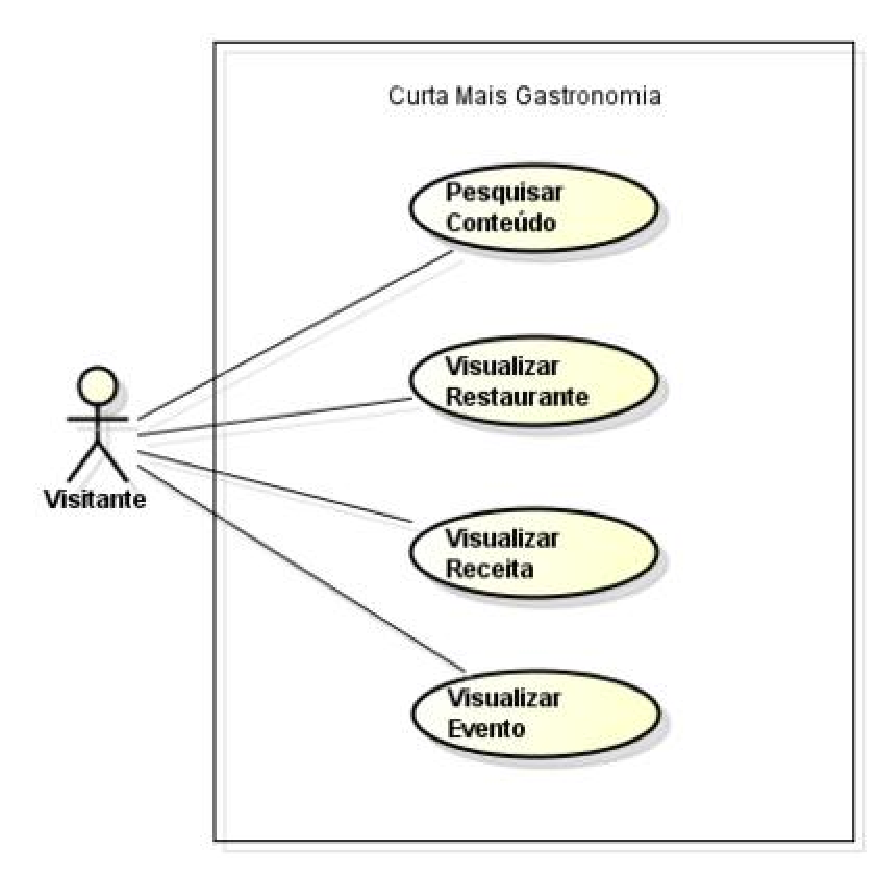
\includegraphics[keepaspectratio,scale=0.6]{figuras/diagrama.eps}
		\caption{Diagrama de Caso de Uso - Gastronomia}
	\end{center}
\end{figure}

\section{Descrição dos Casos de Uso}

\begin{table}[H]
\begin{tabular}{| p{6cm} | p{10cm} |}
	\hline
	\textbf{ID} & UC01\tabularnewline
	\hline
	\hline
	\textbf{Nome do Caso de Uso} & Cadastrar restaurante\tabularnewline
	\hline
	\textbf{Objetivo} & Adicionar um novo restaurante  na aplicação\tabularnewline
	\hline
	\textbf{Ator(es)} & Administrador\tabularnewline
	\hline
	\textbf{Pré-condição} & Estar logado com uma conta de administrador\tabularnewline
	\hline
	\textbf{Pós-condição} & Um novo restaurante é criado no sistema\tabularnewline
	\hline
	\textbf{Fluxo Principal /Básico /Normal} & Esse caso de uso começa quando o administrador seleciona a opção de criar um novo Restaurante:
	\begin{enumerate}
		\item O sistema encaminha o administrador para a tela de cadastro de novo restaurante.
		\item O administrador preenche as informações necessárias para o cadastro do restaurante.
		\item O sistema retorna a informação de que o restaurante foi cadastrado com sucesso.
		\item O administrador é encaminhado pelo sistema à tela do restaurante recém criado.
		\item O caso de uso é encerrado.
	\end{enumerate} \tabularnewline
	\hline
	\textbf{Fluxo Alternativo} & \tabularnewline
	\hline
\end{tabular}
\caption{Descricao dos Casos de Uso - Cadastrar Restaurante}
\label{DCU_Cadastrar_Restaurante}
\end{table}


\begin{table}[H]
\begin{tabular}{| p{6cm} | p{10cm} |}
	\hline
	\textbf{ID} & UC02\tabularnewline
	\hline
	\hline
	\textbf{Nome do Caso de Uso} & Visualizar Restaurante\tabularnewline
	\hline
	\textbf{Objetivo} & Apresentar detalhes de um restaurante para o visitante\tabularnewline
	\hline
	\textbf{Ator(es)} & Visitante\tabularnewline
	\hline
	\textbf{Pré-condição} & Acessar a aplicação\tabularnewline
	\hline
	\textbf{Pós-condição} & \tabularnewline
	\hline
	\textbf{Fluxo Principal /Básico /Normal} & Este caso de uso se inicia quando o visitante seleciona a opção de restaurantes:
	\begin{enumerate}
		\item O visitante clica em uma categoria de restaurante.
		\item O sistema encaminha o visitante para uma lista de restaurantes sob aquela categoria.
		\item O visitante clica no nome de um dos restaurantes listados.
		\item O sistema encaminha o visitante para a página do restaurante selecionado.
		\item Este caso de uso é encerrado.
	\end{enumerate} \tabularnewline
	\hline
	\textbf{Fluxo Alternativo} & \tabularnewline
	\hline
\end{tabular}
\caption{Descricao dos Casos de Uso - Visualizar Restaurante}
\label{DCU_Vizualizar_Restaurante}
\end{table}


\begin{table}[H]
\begin{tabular}{| p{6cm} | p{10cm} |}
	\hline
	\textbf{ID} & UC02\tabularnewline
	\hline
	\hline
	\textbf{Nome do Caso de Uso} & Visualizar Receita\tabularnewline
	\hline
	\textbf{Objetivo} & Apresentar detalhes de uma receita para o visitante\tabularnewline
	\hline
	\textbf{Ator(es)} & Visitante\tabularnewline
	\hline
	\textbf{Pré-condição} & Acessar a aplicação\tabularnewline
	\hline
	\textbf{Pós-condição} & \tabularnewline
	\hline
	\textbf{Fluxo Principal /Básico /Normal} & Este caso de uso se inicia quando o visitante seleciona a opção de restaurantes:
	\begin{enumerate}
		\item O visitante clica em uma categoria de receita.
		\item O sistema encaminha o visitante para uma lista de receitas sob aquela categoria.
		\item O visitante clica no nome de uma das receitas listadas.
		\item O sistema encaminha o visitante para a página da receita selecionada.
		\item Este caso de uso é encerrado.
	\end{enumerate} \tabularnewline
	\hline
	\textbf{Fluxo Alternativo} & \tabularnewline
	\hline
\end{tabular}
\caption{Descricao dos Casos de Uso - Visualizar Receita}
\label{DCU_Visualizar_Receita}
\end{table}